\documentclass[UTF8,a4paper,11pt]{ctexart}
\setCJKmainfont[Path=./,Extension=.otf,BoldFont=NotoSansSC-Bold]{NotoSansSC-Regular}
\usepackage[left=2.55cm,right=2.55cm,top=2.65cm,bottom=2.5cm,headheight=14pt]{geometry}
\usepackage{fancyhdr,graphicx,booktabs,longtable,array,float,xcolor,listings,hyperref,tikz,enumitem,needspace}
\hypersetup{hidelinks}
\emergencystretch=2em
\setlength{\parindent}{2em}\setlength{\parskip}{0pt}\linespread{1.28}
\setlist{topsep=3pt,itemsep=2pt}
\pagestyle{fancy}\fancyhf{}\fancyhead[L]{互联网数据库课程设计}\fancyhead[R]{实现文档}\fancyfoot[C]{\thepage}\renewcommand{\headrulewidth}{0.4pt}
\ctexset{section={format=\zihao{3}\bfseries,beforeskip=15pt,afterskip=9pt},subsection={format=\zihao{4}\bfseries,beforeskip=10pt,afterskip=6pt},subsubsection={format=\zihao{-4}\bfseries,beforeskip=7pt,afterskip=4pt}}
\lstset{basicstyle=\ttfamily\footnotesize,breaklines=true,breakatwhitespace=false,columns=fullflexible,keepspaces=true,frame=single,framerule=.35pt,framesep=5pt,xleftmargin=5pt,xrightmargin=3pt,aboveskip=7pt,belowskip=9pt,showstringspaces=false,tabsize=2}
\renewcommand{\figurename}{图}\renewcommand{\tablename}{表}
\begin{document}
\begin{titlepage}
\thispagestyle{empty}
\centering
\vspace*{0cm}

\includegraphics[width=11.5cm]{coverasset-000.png}\par
\vspace{1.62cm}
{\zihao{2} 互联网数据库课程设计\par}
\vspace{0.85cm}
{\zihao{3} 世界杯宇宙\par}
\vspace{0.78cm}
{\zihao{4} 实现文档\par}
\vspace{6.95cm}
{\zihao{-4} 项目名称: WorldCup Universe\par}
\vfill
{\zihao{-4} 南开大学\par}
\vspace{0.1cm}
\end{titlepage}
\setcounter{page}{1}\tableofcontents\clearpage
\section{项目概况}
世界杯宇宙（WorldCup Universe）是一套基于 Yii2 的世界杯主题网站。网站保存球队、球员、赛程、积分、国家档案和体育新闻，提供资料检索、比赛详情、球迷讨论、个人中心及后台管理。前台采用统一导航和卡片式布局，后台集中维护赛事数据、新闻来源、社区内容及课程资料。

项目使用 PHP 8.1 以上版本和 Yii2 2.0 编写服务器程序，使用 MariaDB 保存业务数据。Nginx、PHP-FPM 承担公网访问，本地开发采用 PHP 内置服务器。前台页面采用 HTML、CSS 和 JavaScript，部分展示组件复用 Arena、Tabler 和 Multiverse 资源。

\Needspace{7\baselineskip}
\subsection{业务模块}
赛事资料包括球队、球员、比赛、积分和晋级关系。新闻模块从 RSS 来源同步文章；球迷论坛保存主题、回复、点赞、收藏、举报和通知。注册用户可以设置主队、关注球队及球员。管理员通过后台维护业务数据和处理社区内容。团队页集中展示成员信息及课程附件。

工程使用 Yii2 原生 MVC 组织页面请求，另设 services 承担跨表事务和来源导入。基础建表语句位于 data/install.sql，migrations 保存数据结构升级，commands 提供安装、官方数据导入及新闻同步命令。
\section{项目工程结构}
浏览器请求由 public/index.php 进入 Yii2 应用。程序读取 config/web.php 中的 URL 规则，调用对应控制器；控制器读取参数、验证身份并调用模型或服务层。页面使用 render 输出 HTML，接口使用 JSON 响应。命令行通过 yii 入口运行 commands 下的任务。

\begin{longtable}{>{\raggedright\arraybackslash}p{.28\textwidth}>{\raggedright\arraybackslash}p{.64\textwidth}}\toprule 项目 & 说明\\\midrule\endfirsthead\toprule 项目 & 说明\\\midrule\endhead
public/ & 唯一 Web 根目录；入口、静态资源、公开上传文件\\\midrule
config/ & Yii2 Web 与 Console 配置、数据库连接、路由及后台注册表\\\midrule
controllers/ & 身份访问控制、页面请求和表单入口\\\midrule
models/ & ActiveRecord 表映射、属性规则与模型关联\\\midrule
services/ & 事务、数据查询、新闻导入、偏好、审计及上传\\\midrule
views/ & 前台页面、管理员页面、通用布局和局部模板\\\midrule
commands/ & 安装、数据导入、审计及新闻同步命令\\\midrule
migrations/ & 数据库结构和展示数据的版本化迁移\\\midrule
data/ & 安装 SQL、体育种子、来源快照及课程材料\\\midrule
scripts/ 与 deploy/ & 生产安装、自动更新、备份及系统服务配置\\\midrule
\bottomrule\caption{主要工程目录}\end{longtable}

\Needspace{16\baselineskip}
\noindent\textbf{public/index.php：Web 入口及 Yii2 启动}\par\vspace{2pt}
\begin{lstlisting}
// Composer 和 Yii2 依赖由同一个公开入口加载
require $vendorAutoload;
require $yiiBootstrap;
require dirname(__DIR__) . '/app/bootstrap.php';
header('X-Backend: Yii2');
$config = require dirname(__DIR__) . '/config/web.php';
(new yii\web\Application($config))->run();
\end{lstlisting}

\Needspace{7\baselineskip}
\subsection{请求分发}
控制层使用 Yii2 自带的 URL Manager 将 /teams、/players、/worldcup、/forum、/admin 等路径分配到对应 action。读取型页面调用查询服务或模型，视图用 render 输出 HTML；需要持久化的提交由服务层访问数据库。业务操作成功后通常重定向到详情页，字段验证失败则返回原表单和错误信息。

前后台共用 Yii2 身份组件与 Session。普通页面采用主布局，后台使用 admin 布局，角色访问控制写在控制器的 behaviors 中。这样既可在控制器入口拒绝越权请求，也能让所有页面使用同一套数据库记录。

\Needspace{16\baselineskip}
\noindent\textbf{config/web.php：核心 URL 路由节选}\par\vspace{2pt}
\begin{lstlisting}
'urlManager' => [
  'enablePrettyUrl' => true,
  'showScriptName' => false,
  'rules' => [
    'teams' => 'team/index',
    'players' => 'player/index',
    'worldcup' => 'match/index',
    'worldcup/standings' => 'match/standings',
    'forum' => 'forum/index',
    'forum/<id:\d+>' => 'forum/view',
    'profile' => 'profile/index',
    'admin' => 'admin/index',
    'api/v1/session' => 'api/session',
  ],
],
\end{lstlisting}
\Needspace{7\baselineskip}
\subsection{应用配置}
数据库连接参数使用 .env 中的 DB\_HOST、DB\_PORT、DB\_DATABASE、DB\_USERNAME 和 DB\_PASSWORD。运行缓存、会话和日志保存在 storage 目录。开发环境可自动生成持久化 Cookie 签名密钥，生产环境在 .env 中设置固定密钥。

Web 配置设置 enableCsrfValidation、HttpOnly 及 SameSite=Lax。生产 HTTPS 地址启用 Secure Cookie。相应安全配置与 AuthController 的明文 HTTP 登录限制相互配合。

\Needspace{16\baselineskip}
\noindent\textbf{config/web.php：会话及 CSRF 配置要点}\par\vspace{2pt}
\begin{lstlisting}
'request' => [
  'cookieValidationKey' => $key,
  'enableCsrfValidation' => true, // 写请求校验令牌
  'csrfCookie' => [
    'httpOnly' => true,
    'secure' => $secure,
    'sameSite' => 'Lax',
  ],
  'parsers' => [
    'application/json' => yii\web\JsonParser::class,
  ],
],
'session' => [
  'name' => 'WCUSESSID',
  'savePath' => $runtime.'/sessions',
  'GCProbability' => 1,
],
\end{lstlisting}
\section{数据库初始结构}
应用使用 InnoDB 关系表保存赛事、账户、社区、新闻和来源记录。基础 SQL 位于 data/install.sql，控制台安装入口执行基础建表、角色初始化和 Yii2 迁移；数据结构的继续扩展由 migration 表记录版本。当前结构包括 47 张业务表和 1 张 Yii2 迁移历史表。

赛事域使用 teams、players、matches、match\_lineups、standings 等表；账号域以 users、roles、user\_roles 保存身份与权限；论坛域使用 forum\_threads、forum\_replies、thread\_likes、thread\_bookmarks、forum\_reports；新闻域通过 news\_sources、news\_articles、tags 与 news\_article\_tags 组织来源和分类。表间引用与业务约束分别由数据库外键和服务层判断。

\Needspace{7\baselineskip}
\subsection{数据库迁移}
开发期间新增了论坛主题与回复、偏好关联、通知、官方导入凭证、回放目录等表。基础结构只负责初始建表，迁移承担新增表、索引与字段变更。升级时 Yii2 按 migration 表记录的历史执行尚未应用的迁移。

官方体育资料采用稳定的标识更新原有实体，防止重新导入改变用户关注和论坛主题所引用的 ID。对于跨多张表的数据写入，使用数据库事务将各表更新一起提交；源文件损坏或字段异常则终止本轮导入。

\Needspace{7\baselineskip}
\subsection{数据库版本}
运行环境推荐 MariaDB 10.4 及以上版本，公网部署使用 MariaDB 10.6。安装 SQL 在长度较大的 utf8mb4 URL 字段上设置唯一索引；项目使用 MariaDB 10.6 运行，长 URL 字段的唯一索引采用其兼容机制。

字段采用 utf8mb4 字符集，保存中文、球员原文姓名和其他多语种信息。赛事查询使用外键关联球队与球员，论坛及新闻使用状态过滤，列表按筛选条件和索引分页读取。


\Needspace{16\baselineskip}
\noindent\textbf{models/RegisterForm.php：注册字段校验和角色写入}\par\vspace{2pt}
\begin{lstlisting}
public function rules(): array
{
    return [
        [['username','email','display_name'],'trim'],
        [['username','email','password'],'required'],
        ['username','match','pattern'=>'/^[a-zA-Z0-9_]{3,40}$/'],
        ['username','unique','targetClass'=>User::class],
        ['email','email'],
        ['email','unique','targetClass'=>User::class],
        ['password','string','min'=>12,'max'=>128],
    ];
}
// register() 内的事务写入密码哈希和普通用户角色
$user->password_hash = password_hash($this->password,PASSWORD_DEFAULT);
if (!$user->save()) { $this->addErrors($user->getErrors()); return null; }
$role = Role::findOne(['name'=>'user']);
Yii::$app->db->createCommand()->insert('user_roles', [
    'user_id'=>$user->id, 'role_id'=>$role->id
])->execute();
\end{lstlisting}

\section{FIFA 数据采集}
体育资料脚本 scripts/fetch\_fifa.py 从登记的 FIFA 公开来源读取赛程接口及参赛名单 PDF，来源域名限制为 api.fifa.com 和 fdp.fifa.org。下载文件保存响应、时间、状态码、字节数及 SHA256，集中存放在 data/official/20261021。

采集脚本将来源数据组织为 normalized.json，并使用 manifest.json 记录文件名、源地址和哈希。名单涵盖 48 支球队，每队 26 名球员；比赛接口记录 104 场比赛的详情。原始文件与规范化结果分开保存，便于逐条比较导入内容与来源。


\Needspace{16\baselineskip}
\noindent\textbf{scripts/fetch\_fifa.py：官方接口请求及来源记录}\par\vspace{2pt}
\begin{lstlisting}
def get(self, url, filename):
    parsed = urllib.parse.urlsplit(url)
    # 只使用登记的 FIFA 官方 HTTPS 域名
    if parsed.scheme != 'https' or parsed.hostname not in {
        'api.fifa.com', 'fdp.fifa.org'
    }:
        raise ValueError('Source host is not in the official allowlist')
    path = self.folder / filename
    meta = path.with_suffix(path.suffix + '.meta.json')
    # 请求响应限制为 12 MB，记录时间、状态和校验码
    req = urllib.request.Request(url, headers={
        'User-Agent':'WorldCupUniverse-Coursework/2.0 (public data research)',
        'Accept':'application/json,application/pdf'
    })
    with urllib.request.urlopen(req, timeout=45) as res:
        payload = res.read(12 * 1024 * 1024 + 1)
        record = {'url':url, 'file':filename,
                  'retrieved_at':dt.datetime.now(dt.timezone.utc).isoformat(),
                  'http_status':res.status,
                  'sha256':hashlib.sha256(payload).hexdigest(),
                  'bytes':len(payload)}
    path.write_bytes(payload)
    meta.write_text(json.dumps(record, indent=2), 'utf-8')
\end{lstlisting}

\Needspace{7\baselineskip}
\subsection{来源文件校验}
导入服务读取 manifest.json，并逐个计算原始文件和 normalized.json 的 SHA256。程序检查 HTTPS 协议、来源主机、HTTP 200 状态和球队、球员、比赛的数量。来源验证成功后开始写入数据库，异常直接抛给调用层。

对于同同一份清单，使用 manifest\_sha256 查询 official\_imports。已保存且解析版本一致的导入可直接复用既有报告，防止重复导入产生新的业务实体。

\Needspace{16\baselineskip}
\noindent\textbf{services/OfficialFifaSyncService.php：来源和文件一致性判断}\par\vspace{2pt}
\begin{lstlisting}
if (!hash_equals($m['normalized_sha256'],
        hash_file('sha256', $dir.'/normalized.json'))) {
    throw new \RuntimeException('Normalized hash mismatch');
}
foreach ($m['sources'] as $s) {
    $u = parse_url($s['url']);
    $path = realpath($dir.'/'.$s['file']);
    // 限制来源主机和文件所在目录
    if (($u['scheme'] ?? '') !== 'https'
        || !in_array($u['host'] ?? '',
            ['api.fifa.com','fdp.fifa.org'], true)
        || $s['http_status'] !== 200
        || !$path || dirname($path) !== $dir
        || !hash_equals($s['sha256'],
            hash_file('sha256', $path))) {
        throw new \RuntimeException('Source evidence validation failed');
    }
}
\end{lstlisting}

\Needspace{16\baselineskip}
\noindent\textbf{scripts/fetch\_fifa.py：名单 PDF 的逐页读取及人数校验}\par\vspace{2pt}
\begin{lstlisting}
def parse_squads(path):
    teams = []
    with pdfplumber.open(path) as pdf:
        if len(pdf.pages) != 48:
            raise ValueError('Expected 48 official squad pages')
        for page_no, p in enumerate(pdf.pages, 1):
            text = p.extract_text()
            heading = re.search(r'^(.+?) \(([A-Z]{3})\)$', text, re.M)
            if not heading:
                raise ValueError('Missing squad heading on page ' + str(page_no))
            players = []
            for line in text.splitlines():
                row = re.match(
                    r'^(\d+) (GK|DF|MF|FW) (.+?) (\d{2}/\d{2}/\d{4})'
                    r'(?: (.*?))? (\d+) (\d+) (\d+)$', line)
                if not row:
                    continue
                number, position, names, dob, club, height, caps, goals = row.groups()
                players.append({
                    'shirt_number': int(number), 'position': position,
                    'listed_names': names.replace('\\x00',''),
                    'birth_date': dt.datetime.strptime(dob,'%d/%m/%Y').date().isoformat(),
                    'club': club or None, 'height_cm': int(height),
                    'caps': int(caps), 'goals': int(goals), 'pdf_page': page_no
                })
            if len(players) != 26 or {p['shirt_number'] for p in players} != set(range(1,27)):
                raise ValueError('Squad row parsing failed on page ' + str(page_no))
\end{lstlisting}

\Needspace{7\baselineskip}
\subsection{赛事数据导入}
完成证据校验后，服务开启数据库事务，在 official\_imports 中登记本轮来源清单及其哈希。接着写入球队、球员、比赛、阵容、积分和晋级边。更新既有球队优先匹配原来的编码或官方 ID；球员则结合官方 ID、所属队伍及球衣号码匹配，尽量保留旧记录的主键。

导入记录附带 official\_import\_id 和 source\_synced\_at。后台人工修改经过验证的体育事实时，会清除相应的核验标记，公开查询只读带有效来源的记录。已有用户偏好和论坛关联因此不必因新的导入而改变外键。

\Needspace{16\baselineskip}
\noindent\textbf{services/OfficialFifaSyncService.php：事务和导入凭证核心语句}\par\vspace{2pt}
\begin{lstlisting}
$hash = hash('sha256', $manifest);
$existing = $this->row('official_imports',
    ['manifest_sha256' => $hash]);
if ($existing &&
    (json_decode($existing['report_json'], true)
        ['parser_version'] ?? 0) === 2) {
    return json_decode($existing['report_json'], true)
        + ['reused' => true]; // 相同快照不重复写入
}
$tx = Yii::$app->db->beginTransaction();
$import = $this->put('official_imports',
    ['manifest_sha256' => $hash], [
        'provider' => 'FIFA',
        'manifest_sha256' => $hash,
        'snapshot_path' => str_replace('\\', '/',
            substr($dir, strlen(Yii::getAlias('@app'))+1)),
        'manifest_json' => new \yii\db\JsonExpression($m),
    ]);
$now = gmdate('Y-m-d H:i:s');
$stamp = ['source_synced_at' => $now,
          'official_import_id' => $import];
\end{lstlisting}
\Needspace{7\baselineskip}
\subsection{赛事数据记录}
比赛比分和阵容记录对应已归档的官方接口响应。导入脚本依据 official\_import\_id 管理比赛统计、事件和球员统计的来源状态，公开页面按来源记录筛选。

\section{球队资料}
球队与球员的列表页面按查询条件组合 ActiveRecord 过滤器。球队页面允许按名称和洲足联筛选，球员页面支持姓名、俱乐部、位置与所属球队筛选。列表采用分页，详情根据实体主键查询所属关系。

球队卡片包含国旗、队名和相关照片；球队详情关联球员阵容与赛事记录。球员详情保存号码、位置、出生日期、身高、俱乐部等已采集属性。部分球员统计字段仍为空值，页面保留已采集字段的内容。

\Needspace{16\baselineskip}
\noindent\textbf{controllers/TeamController.php：球队详情关联查询}\par\vspace{2pt}
\begin{lstlisting}
public function actionView(string $id)
{
    $team=(new CatalogService())->find(Team::class,$id);
    return $this->render('/catalog/team', [
        'model'=>$team,
        // 根据球队 ID 查询经过导入验证的球员
        'players'=>Player::find()->where(['team_id'=>$team->id])
            ->andWhere(['not',['official_import_id'=>null]])
            ->orderBy(['shirt_number'=>SORT_ASC])->all(),
        'matches'=>MatchGame::find()->with(['homeTeam','awayTeam'])
            ->where(['or',['home_team_id'=>$team->id],
                          ['away_team_id'=>$team->id]])
            ->andWhere(['not',['official_import_id'=>null]])
            ->orderBy(['starts_at'=>SORT_ASC])->all(),
    ]);
}
\end{lstlisting}

\begin{figure}[H]
\centering
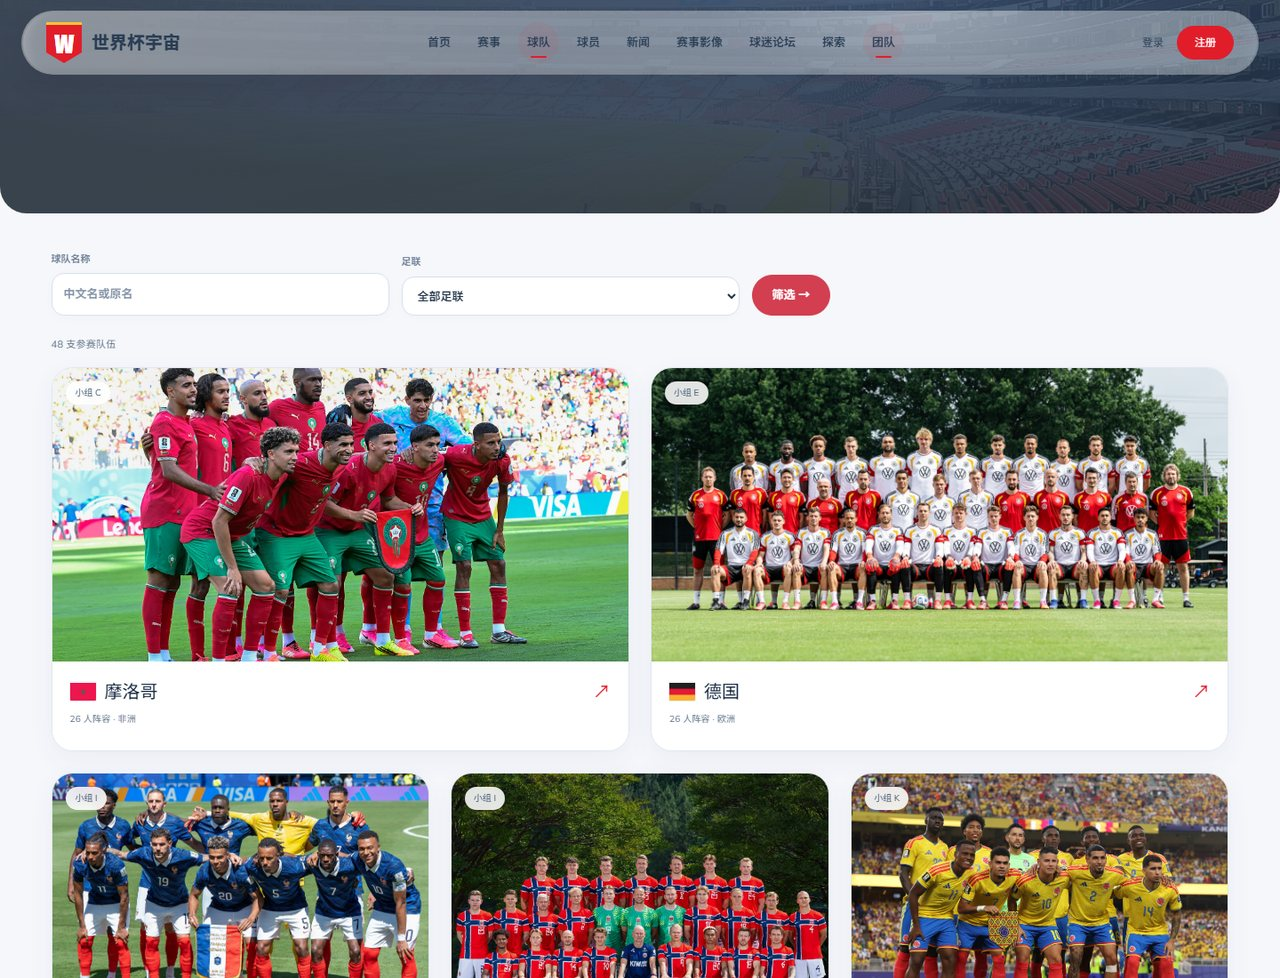
\includegraphics[width=\textwidth]{screenshots/teams.jpg}
\caption{参赛球队页面}
\end{figure}

\begin{figure}[H]
\centering
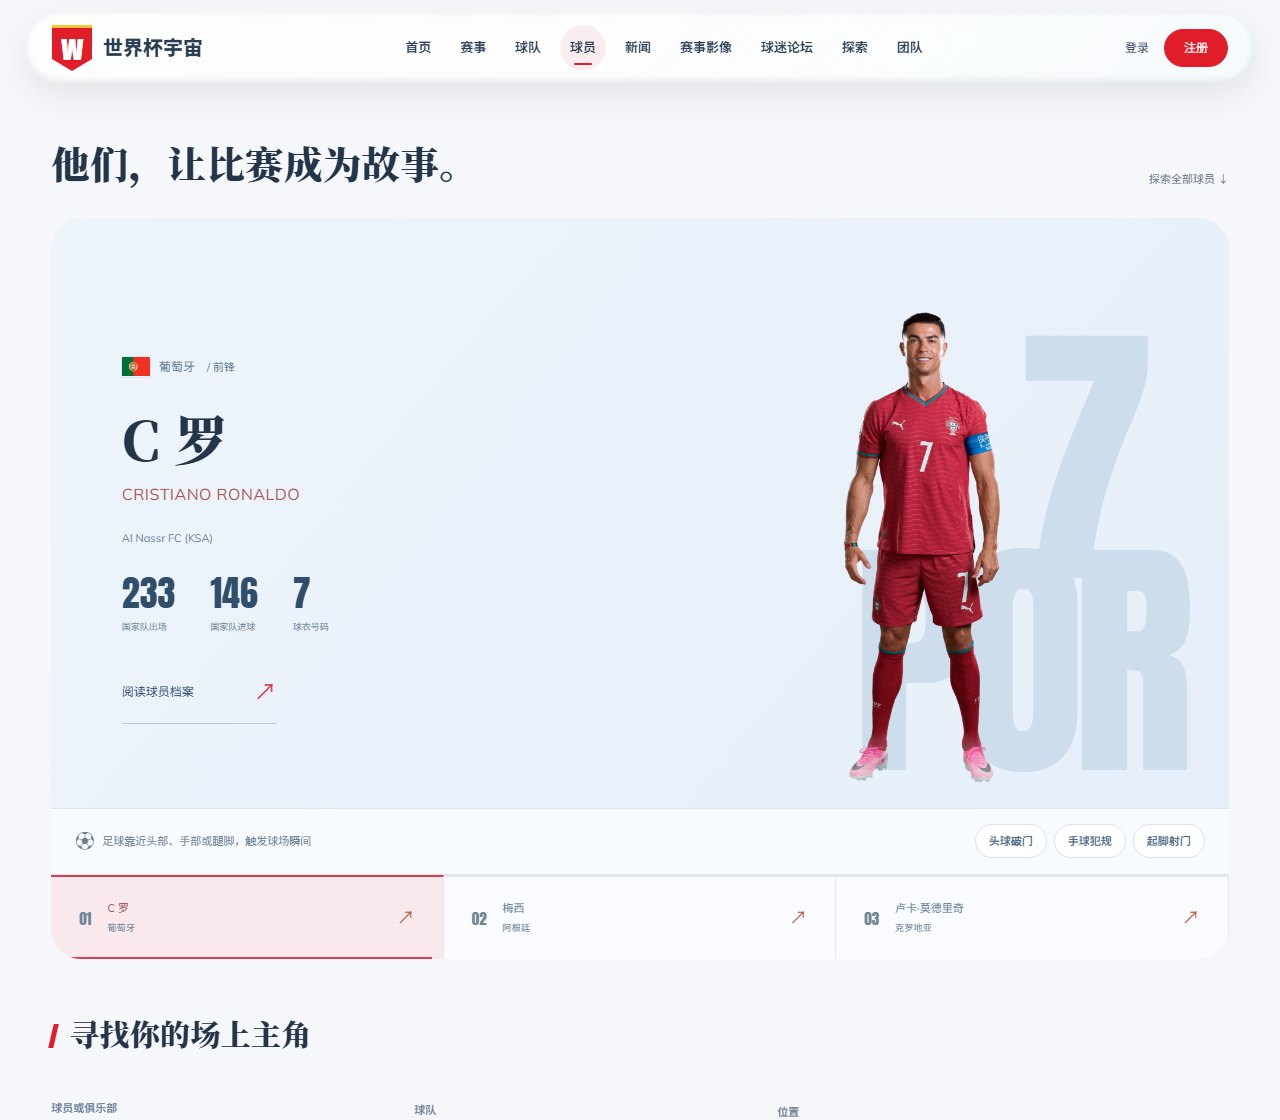
\includegraphics[width=\textwidth]{screenshots/players.jpg}
\caption{球员页面}
\end{figure}

\Needspace{7\baselineskip}
\subsection{赛程及晋级关系}
赛事页以 MatchController 为页面入口。比赛记录使用 home\_team\_id、away\_team\_id 关联球队，使用 starts\_at、stage、status 等条件筛选。小组赛和淘汰赛分别呈现，积分页按 A 至 L 小组组织 standings 数据。

晋级图读取 match\_progressions 中 is\_verified=1 的关系，根据来源比赛、目标比赛、目标位置以及胜者或负者标识组织节点。前端可展开不同轮次；待确定的比赛队伍按照 FIFA 赛程来源保留占位标记。

\Needspace{16\baselineskip}
\noindent\textbf{controllers/MatchController.php：赛程分组及筛选}\par\vspace{2pt}
\begin{lstlisting}
$query=MatchGame::find()->with(['homeTeam','awayTeam'])
    ->where(['not',['official_import_id'=>null]])
    ->orderBy(['starts_at'=>SORT_ASC,'match_number'=>SORT_ASC]);
$query->andFilterWhere([
    'stage'=>Yii::$app->request->get('stage'),
    'status'=>Yii::$app->request->get('status'),
]);
if ($team=Yii::$app->request->get('team_id')) {
    $query->andWhere(['or',
        ['home_team_id'=>$team],['away_team_id'=>$team]]);
}
$groupFixtures=[]; $roundFixtures=[];
foreach ($query->all() as $game) {
    if ($game->stage==='小组赛') {
        $groupFixtures[$game->group_name][]=$game;
    } else { $roundFixtures[$game->stage][]=$game; }
}
ksort($groupFixtures);
\end{lstlisting}

\begin{figure}[H]
\centering
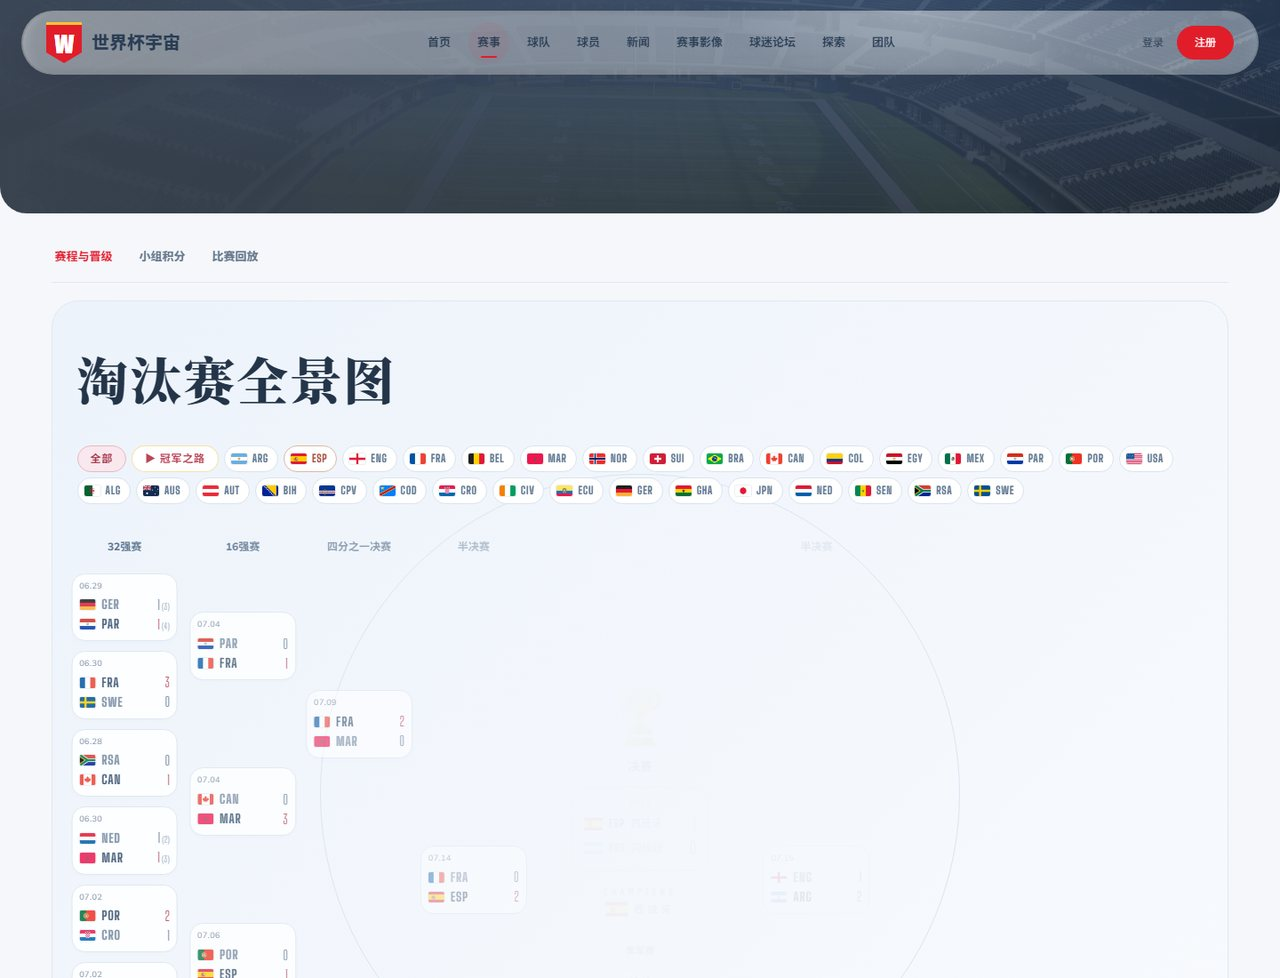
\includegraphics[width=\textwidth]{screenshots/fixtures.jpg}
\caption{赛程与晋级页面}
\end{figure}

\Needspace{7\baselineskip}
\subsection{比赛详情}
进入比赛详情后，通过比赛记录连接双方球队、场馆、阵容、来源和已采集事件。阵容使用 match\_lineups 按所属比赛及球队组织，可能缺少的统计不由客户端推算。比分字段为空的比赛显示待更新状态。

\Needspace{16\baselineskip}
\noindent\textbf{controllers/MatchController.php：比赛详情的关联数据}\par\vspace{2pt}
\begin{lstlisting}
public function actionView(int $id)
{
    // 一次装入双方球队、场馆、统计、事件和阵容
    $model=MatchGame::find()->with([
        'homeTeam','awayTeam','venue',
        'stats.team','events.player','lineups.player'
    ])->where(['id'=>$id])
      ->andWhere(['not',['official_import_id'=>null]])->one();
    if (!$model) { throw new \yii\web\NotFoundHttpException(); }
    return $this->render('/catalog/match',['model'=>$model]);
}
\end{lstlisting}

\section{国家探索}
国家探索页面从 country\_profiles 读取国家代码、坐标、面积、人口、语言与相关摘要，并利用代码与球队资料建立联系。桌面端提供 3D 地球交互，鼠标点击与国家选择联动到详情页面；移动端仍提供普通卡片及语义链接。

三维地球采用 public/assets/js/globe-3d.js 中的交互逻辑。交互地球读取数据库中的国家经纬度、名称及球队关联，国家列表同时保留普通页面链接。

\Needspace{16\baselineskip}
\noindent\textbf{controllers/CountryController.php：国家详情关联参赛球队}\par\vspace{2pt}
\begin{lstlisting}
public function actionView(string $code)
{
    $country=CountryProfile::find()
        ->where(['country_code'=>strtoupper($code)])->asArray()->one();
    if (!$country) {
        throw new \yii\web\NotFoundHttpException('国家资料不存在。');
    }
    $country['linked_teams']=Team::find()
        ->where(['country_code'=>$country['country_code']])
        ->andWhere(['not',['official_import_id'=>null]])
        ->asArray()->all();
    return $this->render('/catalog/country',['country'=>$country]);
}
\end{lstlisting}

\begin{figure}[H]
\centering
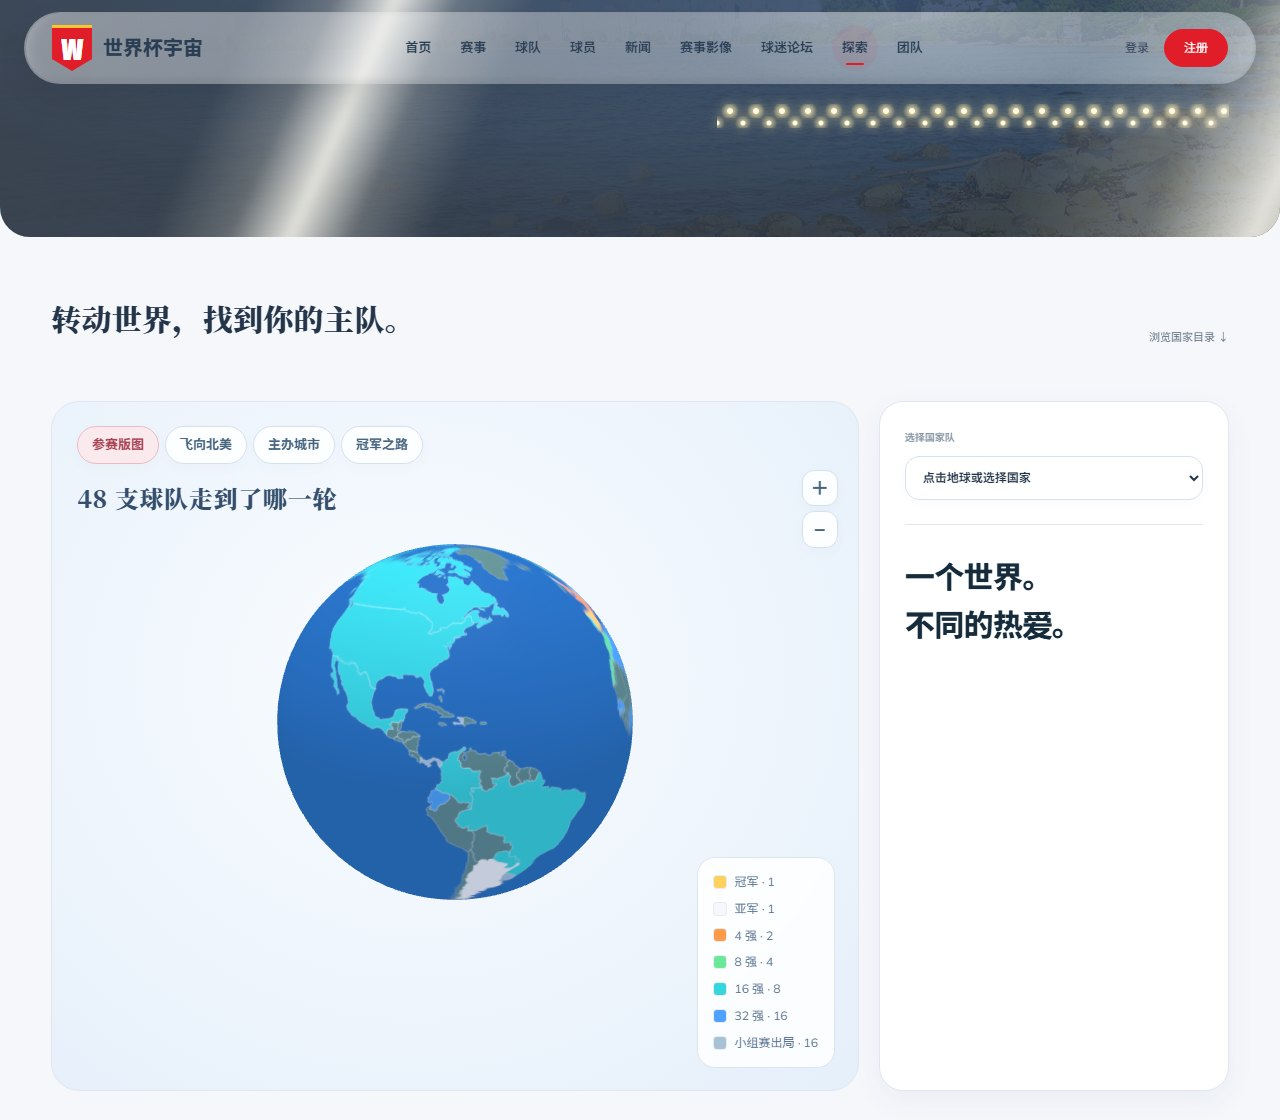
\includegraphics[width=\textwidth]{screenshots/countries.jpg}
\caption{国家探索页面}
\end{figure}

\section{用户注册}
注册控制器使用 RegisterForm 读取 POST 表单并校验字段，随后创建用户、普通角色关联和球迷资料。注册成功后使用 Yii2 用户组件建立登录会话，进入个人中心。用户角色由服务器按照注册流程指定。

用户名采用 3 至 40 位字母、数字和下划线，密码长度为 12 至 128 位；用户名和邮箱设唯一约束。使用 password\_hash 保存密码哈希，登录时通过 password\_verify 校验输入。

\Needspace{16\baselineskip}
\noindent\textbf{controllers/AuthController.php：注册入口实际代码节选}\par\vspace{2pt}
\begin{lstlisting}
public function actionRegister()
{
    if (!Yii::$app->user->isGuest) {
        return $this->redirect('/profile');
    }
    $model = new RegisterForm();
    $insecure = $this->insecure($model, 'password');
    if (!$insecure && Yii::$app->request->isPost
        && $model->load(Yii::$app->request->post())
        && ($user = $model->register())) {
        Yii::$app->user->login($user); // 新账号直接建立会话
        return $this->redirect('/profile');
    }
    $model->password = ''; // 不回填密码字段
    return $this->render('register', [
        'model' => $model, 'insecure' => $insecure
    ]);
}
\end{lstlisting}
\begin{figure}[H]
\centering
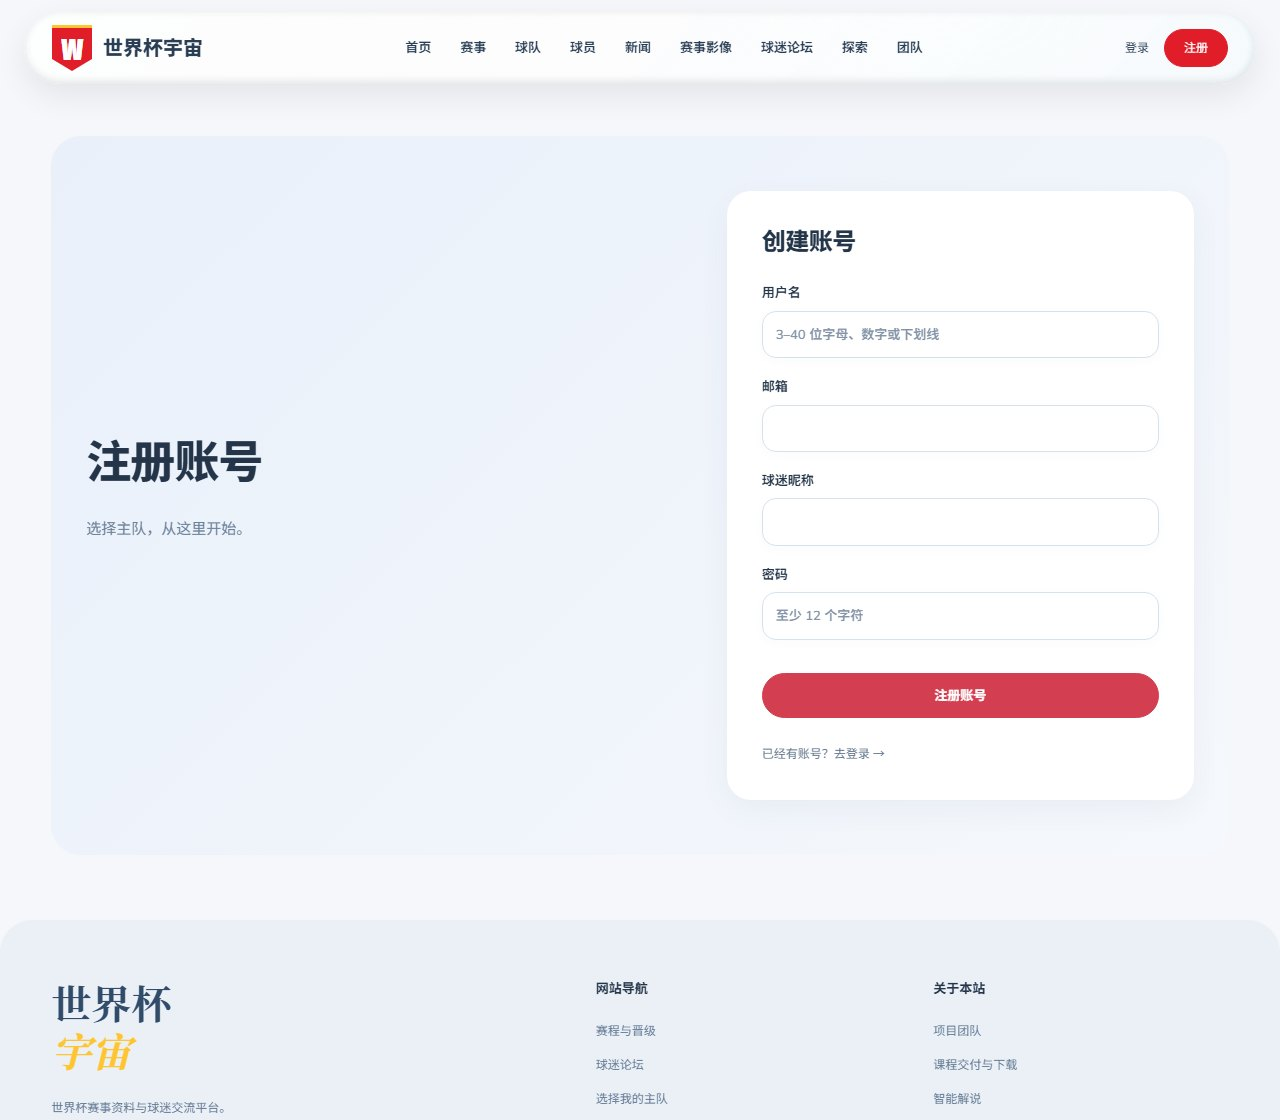
\includegraphics[width=\textwidth]{screenshots/register.jpg}
\caption{账号注册页面}
\end{figure}

\Needspace{7\baselineskip}
\subsection{账号登录}
登录入口使用 LoginForm 验证账号与密码。已登录用户访问登录页直接跳到个人中心，用户退出需要 POST 请求。输入密码的表单不会把原密码回填到页面，避免浏览器继续显示敏感值。

生产环境拒绝通过公网明文 HTTP 登录或注册；本机回环地址与已明确配置的特殊覆盖除外。登录失败的限流机制按用户名和 IP 计数，连续失败达到阈值会暂时限制尝试。账号停用时轮换 auth\_key，使已有会话和记住登录状态失效。


\Needspace{16\baselineskip}
\noindent\textbf{controllers/AuthController.php：登录和退出动作}\par\vspace{2pt}
\begin{lstlisting}
public function actionLogin()
{
    if (!Yii::$app->user->isGuest) {
        return $this->redirect('/profile');
    }
    $model=new LoginForm();
    $insecure=$this->insecure($model,'password');
    if (!$insecure && Yii::$app->request->isPost
        && $model->load(Yii::$app->request->post())
        && $model->login()) {
        return $this->goBack('/profile');
    }
    $model->password='';
    return $this->render('login',[
        'model'=>$model,'insecure'=>$insecure]);
}
public function actionLogout()
{
    $this->posted(); // 退出要求 POST
    Yii::$app->user->logout();
    return $this->goHome();
}
\end{lstlisting}

\begin{figure}[H]
\centering
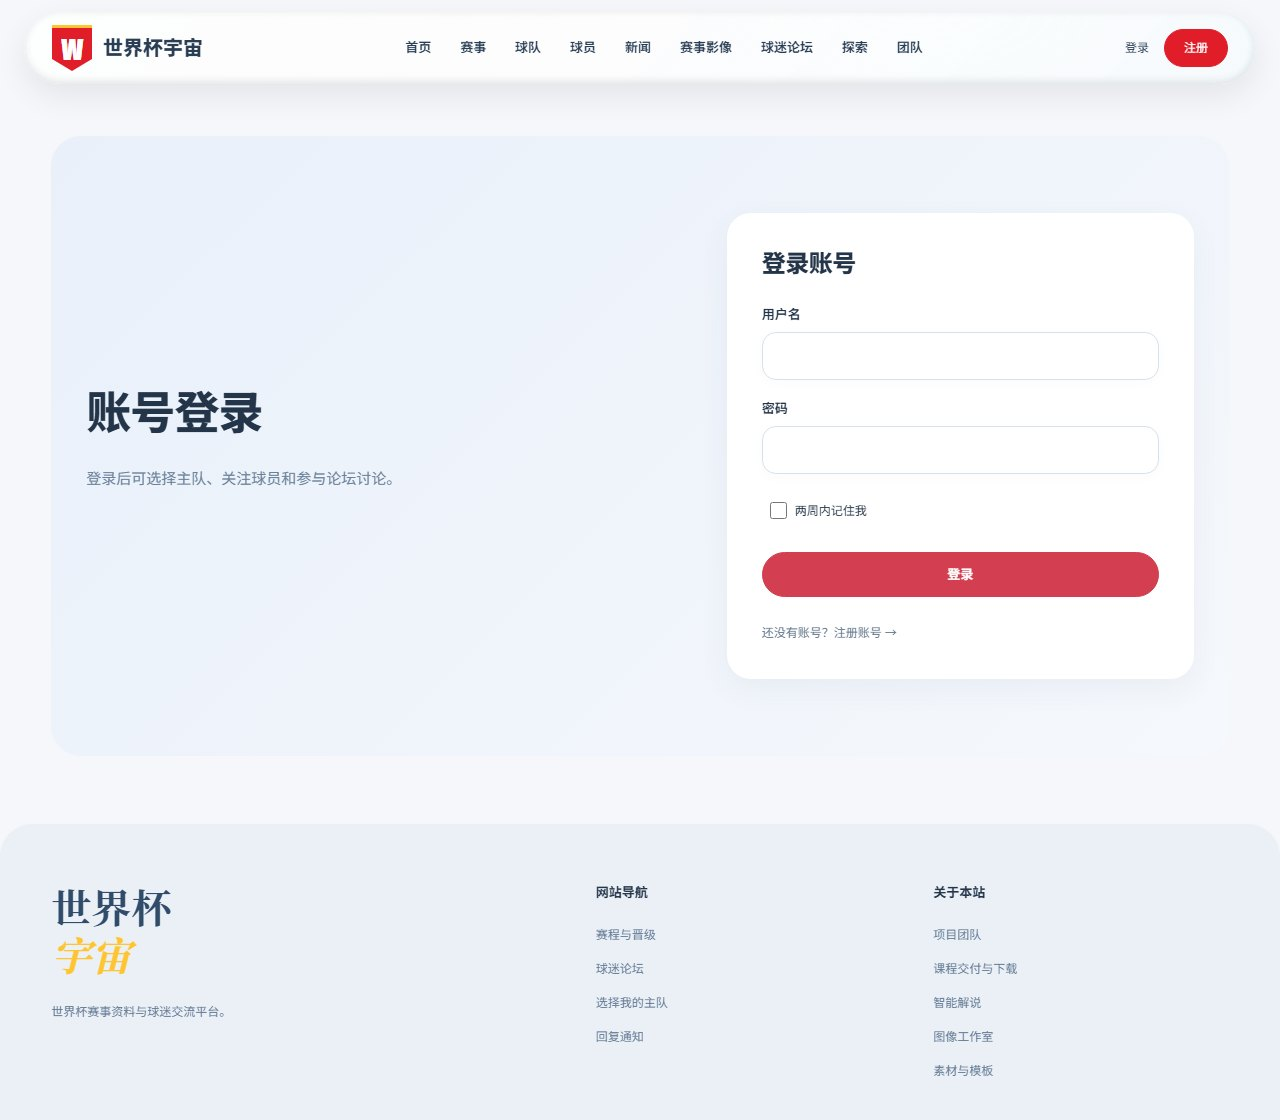
\includegraphics[width=\textwidth]{screenshots/login.jpg}
\caption{账号登录页面}
\end{figure}

\section{个人偏好}
个人中心以 fan\_profiles 保存用户唯一主队，并使用 user\_favorite\_teams、user\_favorite\_players 和 user\_blocked\_teams 保存多选关系。用户选定主队后，服务自动把它加入关注球队；关注和屏蔽集合交叉时，返回字段错误并保持原数据。

保存个人资料时开启数据库事务，更新简介、主队、关注关联和内容偏好。完整保存采用 replace\_preferences=1，将表单中的集合写入关联表；局部更新沿用原有未提交字段。用户 ID 由 Session 中的登录身份确定。

\Needspace{16\baselineskip}
\noindent\textbf{services/PreferenceService.php：主队和关注集合校验}\par\vspace{2pt}
\begin{lstlisting}
$profile = FanProfile::findOne($actor->id)
    ?? new FanProfile();
$profile->user_id = $actor->id;
$profile->setAttributes(array_intersect_key(
    $input, array_flip(['main_team_id','bio'])));
if (!$profile->validate()) { return $profile; }
if ($profile->main_team_id) {
    $teamIds[] = (int)$profile->main_team_id;
}
$teamIds = array_unique($teamIds);
if (array_intersect($teamIds, $blocked)) {
    $profile->addError('main_team_id',
        '主队/关注球队与屏蔽球队不可重叠。');
    return $profile; // 事务尚未执行关联替换
}
\end{lstlisting}
\Needspace{16\baselineskip}
\noindent\textbf{services/PreferenceService.php：关联表替换及订阅保存}\par\vspace{2pt}
\begin{lstlisting}
foreach ([
  'user_favorite_teams'=>['team_id',$teamIds],
  'user_favorite_players'=>['player_id',$playerIds],
  'user_blocked_teams'=>['team_id',$blocked]
] as $table=>[$field,$ids]) {
    // 在同一个数据库事务中重写本人关联
    Yii::$app->db->createCommand()->delete(
        $table,['user_id'=>$actor->id])->execute();
    foreach ($ids as $id) {
        Yii::$app->db->createCommand()->insert($table,[
            'user_id'=>$actor->id,$field=>$id])->execute();
    }
}
Yii::$app->db->createCommand()
    ->upsert('fan_preferences',$prefs)->execute();
\end{lstlisting}

\section{论坛主题的公开列表}
论坛按板块、球队和关键词筛选主题，默认只查询 published 状态。列表同时计算可见回复数和点赞数，并根据置顶、最近活动时间及 ID 排序。页面顶部可进入个人主队讨论和本人发布的主题。

查询通过 ActiveDataProvider 分页，每页 20 条。主题列表预加载作者、主队和分类信息，减少逐条读取关联记录的数据库查询。

\Needspace{16\baselineskip}
\noindent\textbf{controllers/ForumController.php：主题查询与排序}\par\vspace{2pt}
\begin{lstlisting}
$q = ForumThread::find()->alias('t')
    ->with(['author.profile.mainTeam','team','category'])
    ->where(['t.status' => 'published']);
$q->andFilterWhere([
    't.category_id' => Yii::$app->request->get('category'),
    't.team_id' => Yii::$app->request->get('team_id'),
]);
return $this->render('index', [
    'provider' => new ActiveDataProvider([
        'query' => $q->orderBy([
            't.is_pinned' => SORT_DESC,
            't.last_activity_at' => SORT_DESC,
            't.id' => SORT_DESC,
        ]),
        'pagination' => ['pageSize' => 20],
        'sort' => false,
    ]),
]);
\end{lstlisting}
\begin{figure}[H]
\centering
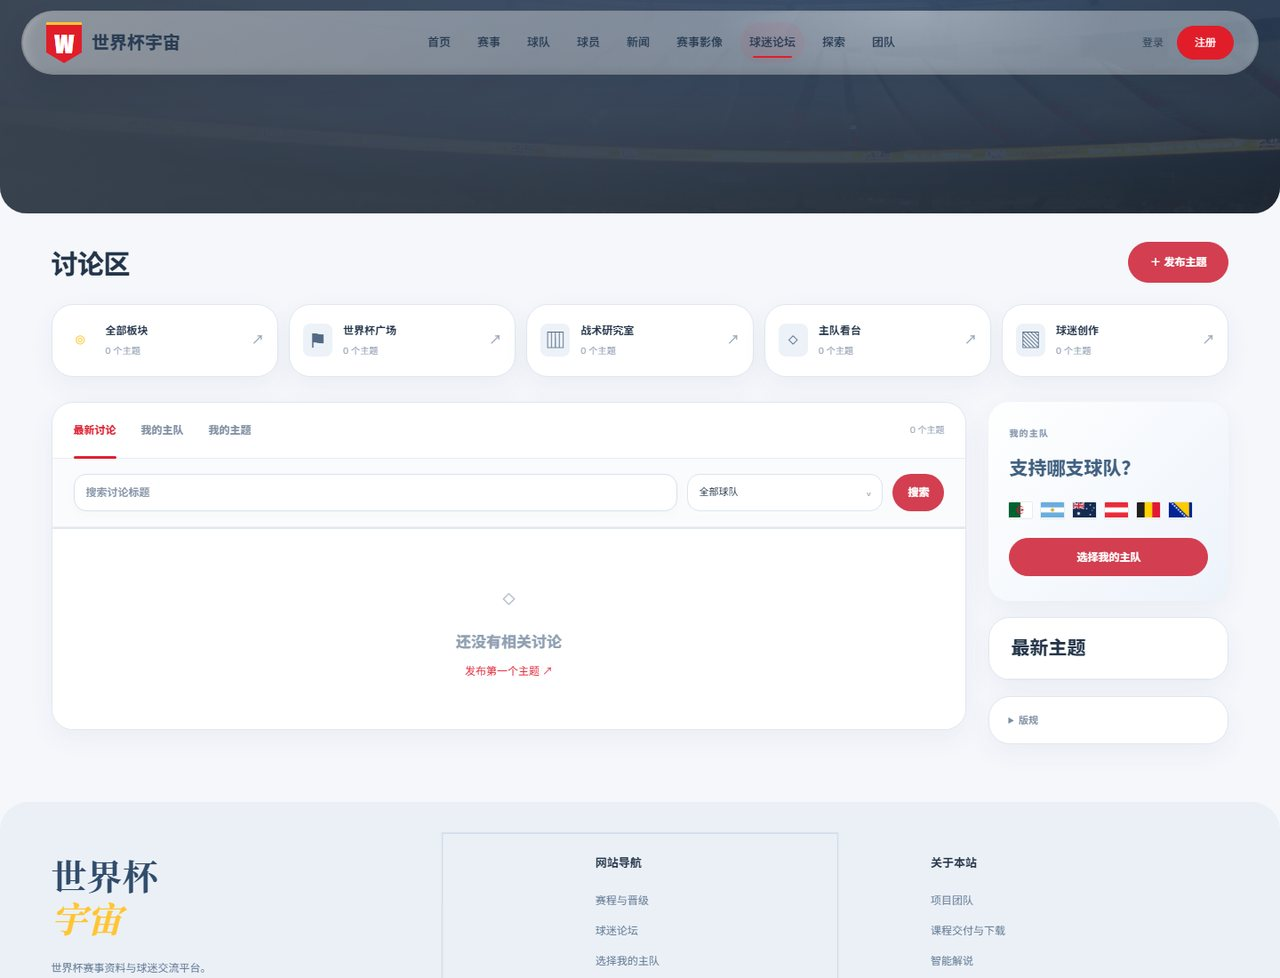
\includegraphics[width=\textwidth]{screenshots/forum.jpg}
\caption{球迷论坛页面}
\end{figure}

\Needspace{7\baselineskip}
\subsection{主题发布}
创建主题时由控制器读取标题、正文、板块及可选球队和比赛 ID。服务层只接收允许的字段，强制使用当前登录身份填写 author\_id，并将新主题状态设置为 published。创建主题有每分钟 5 次的数量限制。

编辑既有主题需要校验作者身份，管理员可以按服务规则修改。删除采用 status=deleted 的软删除方式，保留回复引用和审计关系。对隐藏或锁定主题的普通用户编辑行为，服务层拒绝写入。


\Needspace{16\baselineskip}
\noindent\textbf{services/ForumService.php：发帖字段限制及作者归属}\par\vspace{2pt}
\begin{lstlisting}
return Yii::$app->db->transaction(function () use ($actor,$input,$id) {
    $thread=$id?$this->lockedThread($id):new ForumThread();
    if ($id) { $this->assertOwner($actor,(int)$thread->author_id); }
    // 白名单仅包含用户实际可编辑的业务字段
    $thread->setAttributes(array_intersect_key($input,array_flip([
        'title','body','category_id','team_id','match_id'
    ])));
    if (!$id) {
        $thread->author_id=$actor->id;
        $thread->status='published';
        $thread->last_activity_at=date('Y-m-d H:i:s');
    }
    if ($thread->save()) {
        AuditService::record($id?'thread.update':'thread.create',
                             'forum_threads',(int)$thread->id);
    }
    return $thread;
});
\end{lstlisting}

\Needspace{7\baselineskip}
\subsection{论坛回复}
回复操作先锁定论坛主题行，验证主题为 published 且未锁定，读取正文与可选 parent\_id。引用目标必须属于同一个主题且状态为 visible。服务把回复、主题最后活动时间、通知及审计记录一起写入数据库事务。

通知接收人由主题作者和引用回复作者组成，使用去重集合消除同一用户的重复通知，并跳过当前回复者。通知记录包含收件人、操作者、主题、reply 类型和未读状态。每名用户每分钟最多创建 20 条回复。

\Needspace{16\baselineskip}
\noindent\textbf{services/ForumService.php：事务内写入回复及通知}\par\vspace{2pt}
\begin{lstlisting}
return Yii::$app->db->transaction(function ()
    use ($actor, $threadId, $input) {
    $thread = $this->lockedThread($threadId);
    if ($thread->status !== 'published' || $thread->is_locked) {
        throw new ForbiddenHttpException('主题已锁定或已隐藏。');
    }
    $reply = new ForumReply();
    $reply->setAttributes(array_intersect_key($input,
        array_flip(['body','parent_id'])));
    $reply->thread_id = $thread->id;
    $reply->user_id = $actor->id;
    $reply->status = 'visible';
    $parent = null;
    if ($reply->parent_id) {
        $parent = ForumReply::findOne([
            'id' => $reply->parent_id,
            'thread_id' => $threadId,
            'status' => 'visible',
        ]);
        if (!$parent) {
            throw new BadRequestHttpException(
                '引用回复不属于当前主题。');
        }
    }
    if (!$reply->save()) { return $reply; }
    $thread->last_activity_at = date('Y-m-d H:i:s');
    $thread->save(false);
    $recipients = array_unique([
        (int)$thread->author_id,
        (int)($parent->user_id ?? 0),
    ]);
    foreach ($recipients as $recipient) {
        if ($recipient && $recipient !== (int)$actor->id) {
            Yii::$app->db->createCommand()->insert(
                'notifications', [
                    'user_id' => $recipient,
                    'actor_id' => $actor->id,
                    'thread_id' => $threadId,
                    'type' => 'reply',
                ])->execute();
        }
    }
    AuditService::record('reply.create',
        'forum_replies', (int)$reply->id);
    return $reply;
});
\end{lstlisting}
\Needspace{7\baselineskip}
\subsection{论坛互动}
论坛点赞和收藏分别记录 thread\_likes 与 thread\_bookmarks。二者以用户和主题的联合键保持唯一，同一用户重复设置不产生多份关系。取消操作直接删除对应关联记录。私人收藏列表只读取当前登录用户的记录。

举报记录包含主题、可选回复、举报人、理由和处理状态。创建举报前判断对象是否属于所选主题，并阻止对同一未处理对象重复提交。管理员可对举报作 resolved 或 dismissed 标记，内容隐藏、锁定和举报处理属于不同的审核动作。


\Needspace{16\baselineskip}
\noindent\textbf{services/ForumService.php：点赞收藏及举报记录}\par\vspace{2pt}
\begin{lstlisting}
public function setCollection(User $actor,int $id,
                              string $kind,bool $enabled): void
{
    $this->readable($id,$actor);
    $table=match($kind) {
        'like'=>'thread_likes',
        'bookmark'=>'thread_bookmarks',
        default=>throw new BadRequestHttpException()
    };
    $key=['thread_id'=>$id,'user_id'=>$actor->id];
    if ($enabled) {
        // 联合主键与 upsert 避免重复点赞或收藏
        Yii::$app->db->createCommand()->upsert($table,$key,false)->execute();
    } else {
        Yii::$app->db->createCommand()->delete($table,$key)->execute();
    }
}
\end{lstlisting}

\section{后台管理}
管理入口使用 AdminController 和 admin 布局。通过 AccessControl 的 matchCallback 检查 isAdmin，管理员身份验证通过后进入球队、球员、比赛、新闻、媒体及课程文件的管理列表。

通用管理表单根据 registry 登记项选择 ActiveRecord 类，并按字段规则保存记录。论坛主题、回复和举报通过专用审核入口修改状态，保留内容作者及历史审核信息。

\Needspace{16\baselineskip}
\noindent\textbf{controllers/AdminController.php：管理员准入规则}\par\vspace{2pt}
\begin{lstlisting}
public $layout = 'admin';
public function behaviors(): array
{
    return ['access' => [
        'class' => AccessControl::class,
        'rules' => [[
            'allow' => true,
            'roles' => ['@'],
            'matchCallback' => fn() =>
                Yii::$app->user->identity->isAdmin(),
        ]],
    ]];
}
\end{lstlisting}
\Needspace{7\baselineskip}
\subsection{社区审核}
管理员可以隐藏、恢复和锁定主题，处理举报，并在用户管理界面启用或停用普通账号。改变账号状态时重新生成 auth\_key，使旧会话失效；管理员身份的账号状态由专用维护方式管理。

重要写入调用 AuditService，记录操作类型、业务实体和 ID，供 /admin/audit 只读查询。审计页面按记录时间和操作类型列出历史操作。涉及数据库外键限制的删除操作捕获完整性异常，提示仍被其他记录引用。


\Needspace{16\baselineskip}
\noindent\textbf{services/ForumService.php：审核动作及审计记录}\par\vspace{2pt}
\begin{lstlisting}
if (!$actor->isAdmin()) { throw new ForbiddenHttpException(); }
Yii::$app->db->transaction(function () use ($type,$id,$operation) {
    $class=match($type) {
      'thread'=>ForumThread::class,'reply'=>ForumReply::class,
      'report'=>ForumReport::class,
      default=>throw new BadRequestHttpException()
    };
    $model=$class::findOne($id);
    if (!$model) { throw new NotFoundHttpException(); }
    if ($type==='thread' && in_array($operation,
                    ['lock','unlock','pin','unpin'],true)) {
        $field=in_array($operation,['lock','unlock'],true)
            ?'is_locked':'is_pinned';
        $model->$field=in_array($operation,['lock','pin'],true)?1:0;
    }
    $model->save(false);
    AuditService::record('moderation.'.$operation,
                         $model::tableName(),$id);
});
\end{lstlisting}

\Needspace{7\baselineskip}
\subsection{媒体上传}
后台允许上传登记字段对应的图片、视频与课程资料。上传服务按扩展名和真实 MIME 类型限制文件，并使用随机文件名写入目标目录。公开媒体存放于 public/uploads，课程附件存放在 data/team 或 data/personal 的受控目录。

上传内容的路径由服务器生成，通过随机文件名组织上传文件。后台修改课程文件记录的可见状态后，前台列表据此决定是否显示下载入口。


\Needspace{16\baselineskip}
\noindent\textbf{services/MediaUploadService.php：上传类型及大小配置}\par\vspace{2pt}
\begin{lstlisting}
private const KINDS = [
  'image'=>[
    'ext'=>['jpg'=>['image/jpeg'],'png'=>['image/png'],
            'webp'=>['image/webp']],
    'env'=>'UPLOAD_MAX_IMAGE_MB','mb'=>10
  ],
  'video'=>[
    'ext'=>['mp4'=>['video/mp4','application/mp4'],
            'webm'=>['video/webm','audio/webm']],
    'env'=>'UPLOAD_MAX_VIDEO_MB','mb'=>200
  ],
];
// 实际服务还登记课程文档的扩展名和 MIME 白名单
public static function limitBytes(string $kind): int
{
    $spec=self::kind($kind);
    $mb=(int)env($spec['env'],$spec['mb']);
    return max(1,min(2048,$mb))*1048576;
}
\end{lstlisting}

\section{新闻来源同步}
新闻同步通过 NewsImportService 访问启用的 RSS/Atom 来源。同步开始先获取 FileMutex 锁，防止管理员刷新、后台定时器和 Windows worker 同时改写新闻记录。服务按来源逐个抓取和解析，新闻原文链接作为去重依据。

中国新闻网体育源属于综合体育频道，程序依据标题内容筛选足球报道；其他启用来源由注册列表限定。抓取成功后保存原标题、摘要、发布时间、原文地址、标签和源文件 SHA256，失败来源则写入 last\_error，其他来源继续同步。

\Needspace{16\baselineskip}
\noindent\textbf{services/NewsImportService.php：锁与来源隔离}\par\vspace{2pt}
\begin{lstlisting}
$mutex = new \yii\mutex\FileMutex(['fileMode' => 0664]);
if (!$mutex->acquire('news-import')) {
    return ['saved' => 0, 'updated' => 0,
            'busy' => true, 'sources' => []];
}
$result = ['saved' => 0, 'updated' => 0,
           'curated' => 0, 'sources' => []];
try {
    $this->ensureFootballSources();
    foreach (NewsSource::find()
             ->where(['is_enabled' => 1])->all() as $source) {
        try {
            $xml = $this->fetch((string)$source->rss_url);
            $items = $this->parse($xml);
            $folder = ROOT_PATH.'/storage/source_snapshots/news';
            if (!is_dir($folder)) mkdir($folder, 0775, true);
            file_put_contents($folder.'/source-'.$source->id.'.xml',
                $xml, LOCK_EX);
        } catch (\Throwable $e) {
            $source->last_error = mb_substr(
                $e->getMessage(), 0, 1000);
            $source->save(false);
        }
    }
} finally {
    $mutex->release('news-import');
}
\end{lstlisting}
\Needspace{7\baselineskip}
\subsection{新闻列表}
公开新闻页只读取 published 状态的记录，并支持关键词、来源和标签过滤。页面保留标题、摘要、发布时间和原文入口，用户可以跳到来源网站继续阅读。新闻摘要的中文翻译依赖外部服务配置，源文标题和摘要仍可正常呈现。

生产环境使用定时器执行新闻同步，README 给出的配置周期为每 10 分钟。普通用户打开新闻页时直接查询数据库中的文章。管理员可在后台触发刷新，服务器定时器也会按计划同步来源。


\Needspace{16\baselineskip}
\noindent\textbf{services/CatalogService.php：新闻筛选及来源交错排序}\par\vspace{2pt}
\begin{lstlisting}
$q=NewsArticle::find()->with('tags')
    ->where(['news_articles.status'=>'published'])
    ->orderBy(['news_articles.published_at'=>SORT_DESC]);
if (empty($filters['q']) && empty($filters['source'])) {
    // 按新闻来源分别排名，再交错读取各来源的新文章
    $rank=(new \yii\db\Query())->select([
        'id','source_rank'=>new Expression(
          'ROW_NUMBER() OVER (PARTITION BY source_id '
          .'ORDER BY published_at DESC,id DESC)')
    ])->from('news_articles')->where(['status'=>'published']);
    $q->leftJoin(['feed_rank'=>$rank],
                 'feed_rank.id=news_articles.id')
      ->orderBy(['feed_rank.source_rank'=>SORT_ASC,
                 'news_articles.published_at'=>SORT_DESC]);
}
\end{lstlisting}

\begin{figure}[H]
\centering
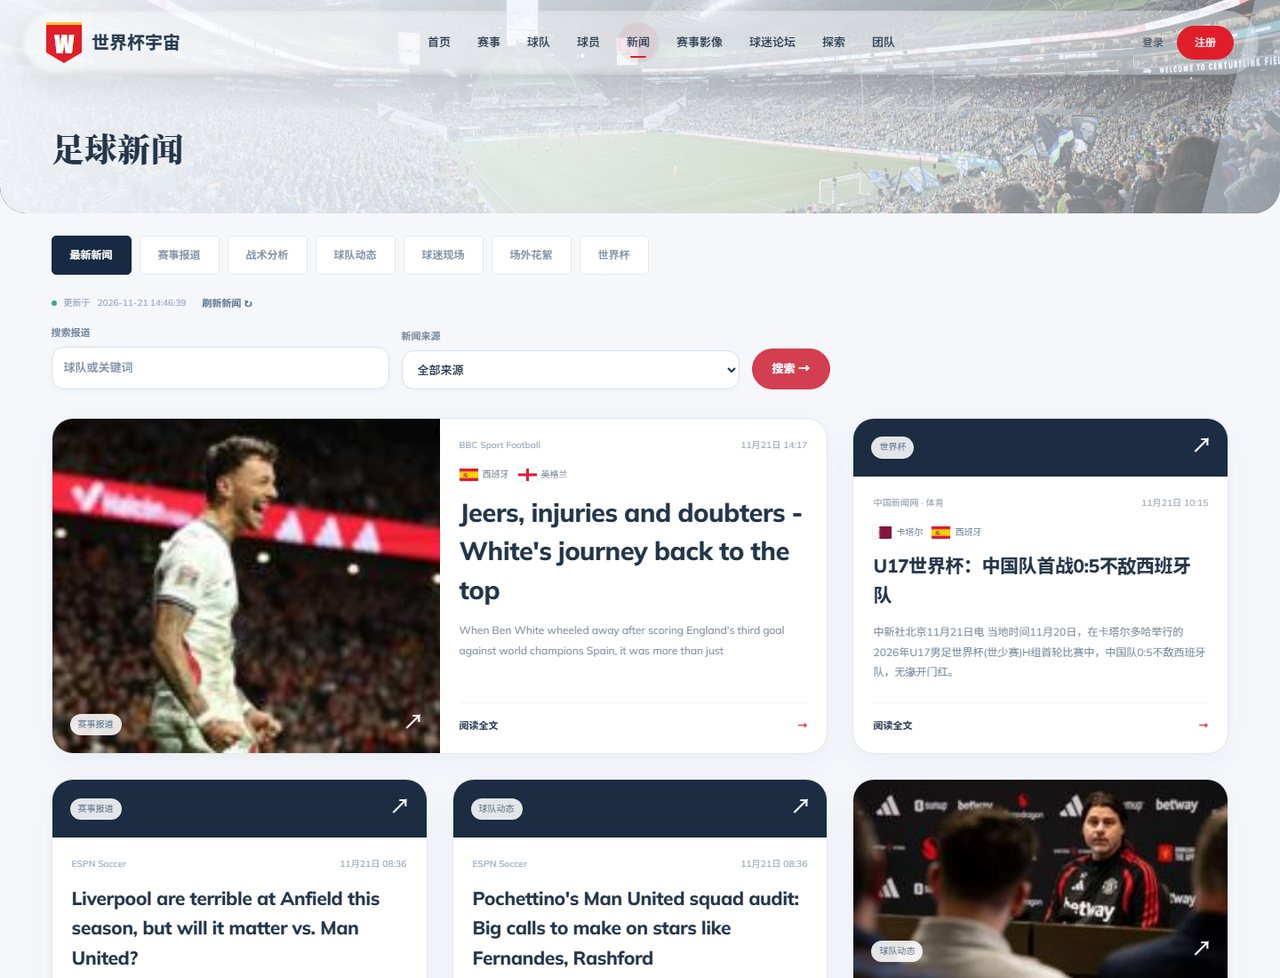
\includegraphics[width=\textwidth]{screenshots/news.jpg}
\caption{足球新闻页面}
\end{figure}

\section{比赛回放}
视频页面由 VideoController 管理，回放来源以经过核验的 2026 年完整比赛目录为准。项目以央视网等官方授权入口为播放来源，第三方播放器可能受到地区和账号条件限制。视频记录保留播放来源和对应比赛元数据。

媒体列表与外部播放器分开管理。公开授权短片通过本地视频文件目录提供，播放过程中官方回放使用明确登记的播放器来源。

\Needspace{16\baselineskip}
\noindent\textbf{controllers/VideoController.php：回放资源选择}\par\vspace{2pt}
\begin{lstlisting}
$official=is_file(ROOT_PATH.'/config/cctv-videos.php')
    ? require ROOT_PATH.'/config/cctv-videos.php' : [];
$library=(new \app\services\LocalVideoLibrary())->all();
$clipSlug=(string)Yii::$app->request->get('clip',$slug??'');
$selected=null;
foreach ($official as $item) {
    if ($item['slug']===$clipSlug || (!$clipSlug && $selected===null)) {
        $selected=$item;
        if ($clipSlug) { break; }
    }
}
if (!$selected && $clipSlug) {
    $selected=(new \app\services\LocalVideoLibrary())->find($clipSlug);
}
return $this->render('/catalog/videos',[
    'official'=>$official,'library'=>$library,'selected'=>$selected
]);
\end{lstlisting}

\begin{figure}[H]
\centering

\includegraphics[width=\textwidth]{screenshots/video.jpg}
\caption{赛事影像页面}
\end{figure}

\Needspace{7\baselineskip}
\subsection{智能解说}
登录用户可输入解说主题、语气及目标球队，调用配置的外部模型生成文字；勾选生图选项后可以发起图片生成请求。模型凭据由服务器环境配置，页面显示实际接口调用状态。

图像页面接收 JPG、JPEG、PNG、WebP 格式文件，按照文件大小及像素限制校验输入，再保存到私有目录。页面提示图片已接收，当前提供图片存储和访问管理功能。


\Needspace{16\baselineskip}
\noindent\textbf{controllers/AiController.php：智能解说请求}\par\vspace{2pt}
\begin{lstlisting}
$model=new AiForm(['scenario'=>'chat']);
$ark=new ArkClient(); $result=null; $image=null;
if (Yii::$app->request->isPost) {
    $actor=$this->actor();
    $this->limit((int)$actor->id);
    if ($model->load(Yii::$app->request->post())
        && $model->validate()) {
        if (!$ark->textReady()) {
            $model->addError('prompt','文本模型尚未配置。');
        } else {
            $result=$ark->chat($model->prompt,
                $model->tone,$model->target_team?:null,60,2000);
            $this->record('chat',$model->prompt,$result);
        }
    }
}
\end{lstlisting}

\section{团队页面}
/team 页面展示项目成员和课程材料，后台管理 coursework\_files 表登记文件名称、范围、路径和前台可见状态。下载控制器限制文件路径位于 data/team 和 data/personal 目录，并通过服务端 sendFile 返回实际文件。

团队文件存放在 data/team，个人文件存放在 data/personal。管理员通过课程交付记录维护文件名称、显示状态及下载入口。


\Needspace{16\baselineskip}
\noindent\textbf{controllers/SiteController.php：团队成员和下载文件}\par\vspace{2pt}
\begin{lstlisting}
public function actionTeam(): string
{
    return $this->render('team', [
        'members'=>\app\models\TeamMember::find()
            ->where(['is_visible'=>1])
            ->orderBy(['sort_order'=>SORT_ASC,'id'=>SORT_ASC])->all(),
        'files'=>(new \app\services\CourseworkLibrary())->grouped(),
        'team'=>require ROOT_PATH.'/config/team.php'
    ]);
}
public function actionDownloadFile(string $scope,string $name)
{
    $path=\app\services\CourseworkLibrary::resolve($scope,$name);
    if (!$path) { Yii::$app->response->statusCode=404;
        return $this->render('error',['status'=>404,
                       'message'=>'文件不存在。']); }
    return Yii::$app->response->sendFile(
        $path,basename($path),['inline'=>false]);
}
\end{lstlisting}

\begin{figure}[H]
\centering
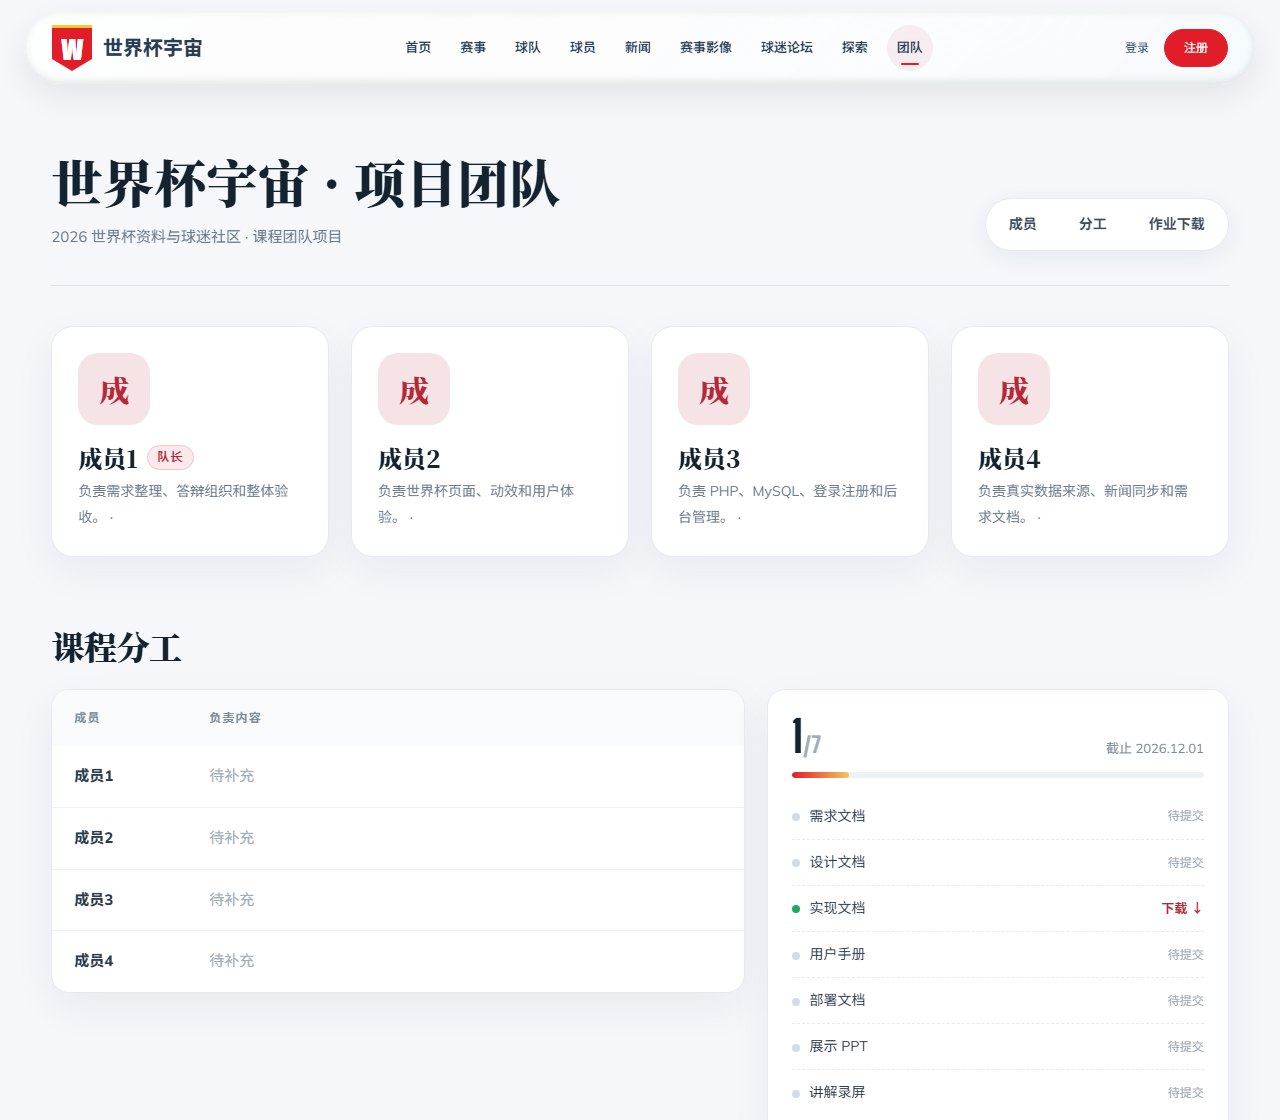
\includegraphics[width=\textwidth]{screenshots/team.jpg}
\caption{团队页面}
\end{figure}

\Needspace{7\baselineskip}
\subsection{JSON 接口}
系统使用 /api/v1 作为 JSON 前缀，页面与接口共用 Yii2 的身份组件、模型和数据服务。只读入口覆盖球队、球员、比赛、积分、新闻、国家及论坛，写入入口检查登录状态与 CSRF。

列表输出包含 data 数组和 pagination.total、page、pageSize，详情接口则返回 data 对象。分页参数从 1 开始，参数格式错误的请求返回 4xx 状态，体育列表按照官方导入标识筛选记录。

\Needspace{16\baselineskip}
\noindent\textbf{docs/v2-api.md：使用本站会话发起 JSON 请求}\par\vspace{2pt}
\begin{lstlisting}
const { data: session } = await fetch('/api/v1/session', {
  credentials: 'same-origin'
}).then(r => r.json());
const response = await fetch('/api/v1/forum', {
  method: 'POST',
  credentials: 'same-origin',
  headers: {
    'Content-Type': 'application/json',
    'X-CSRF-Token': session.csrfToken,
  },
  body: JSON.stringify({
    title: '比赛讨论',
    body: '你如何看待本场的阵容安排？',
    category_id: 1
  }),
});
const result = await response.json();
if (!response.ok) throw new Error(JSON.stringify(result));
\end{lstlisting}

\Needspace{16\baselineskip}
\noindent\textbf{controllers/ApiController.php：JSON 接口统一返回格式}\par\vspace{2pt}
\begin{lstlisting}
public function beforeAction($action): bool
{
    Yii::$app->response->format=Response::FORMAT_JSON;
    return parent::beforeAction($action);
}
public function actionTeams(): array
{
    return $this->page(
        (new CatalogService())->teams(Yii::$app->request->get()));
}
private function page(ActiveDataProvider $p): array
{
    return ['data'=>$this->arrays($p->getModels()),
      'pagination'=>[
        'total'=>$p->getTotalCount(),
        'page'=>$p->pagination->page+1,
        'pageSize'=>$p->pagination->pageSize
      ]];
}
\end{lstlisting}

\section{前台布局}
主布局为各栏目提供顶部导航、页脚和统一的字体现示。赛事页用比赛卡片与分组折叠组织较长赛程；球队及球员卡片在窄屏中调整列数，保留详情链接。多语言名称和图片来源由记录字段控制。

前台部分交互依赖 JavaScript，国家页中的 3D 地球对 WebGL 有要求；与其平行的国家列表链接仍可用于普通浏览器。项目复用 Arena、Tabler 和 Multiverse 的样式组件，并在站点资源中保存相关字体和脚本。

\begin{figure}[H]
\centering
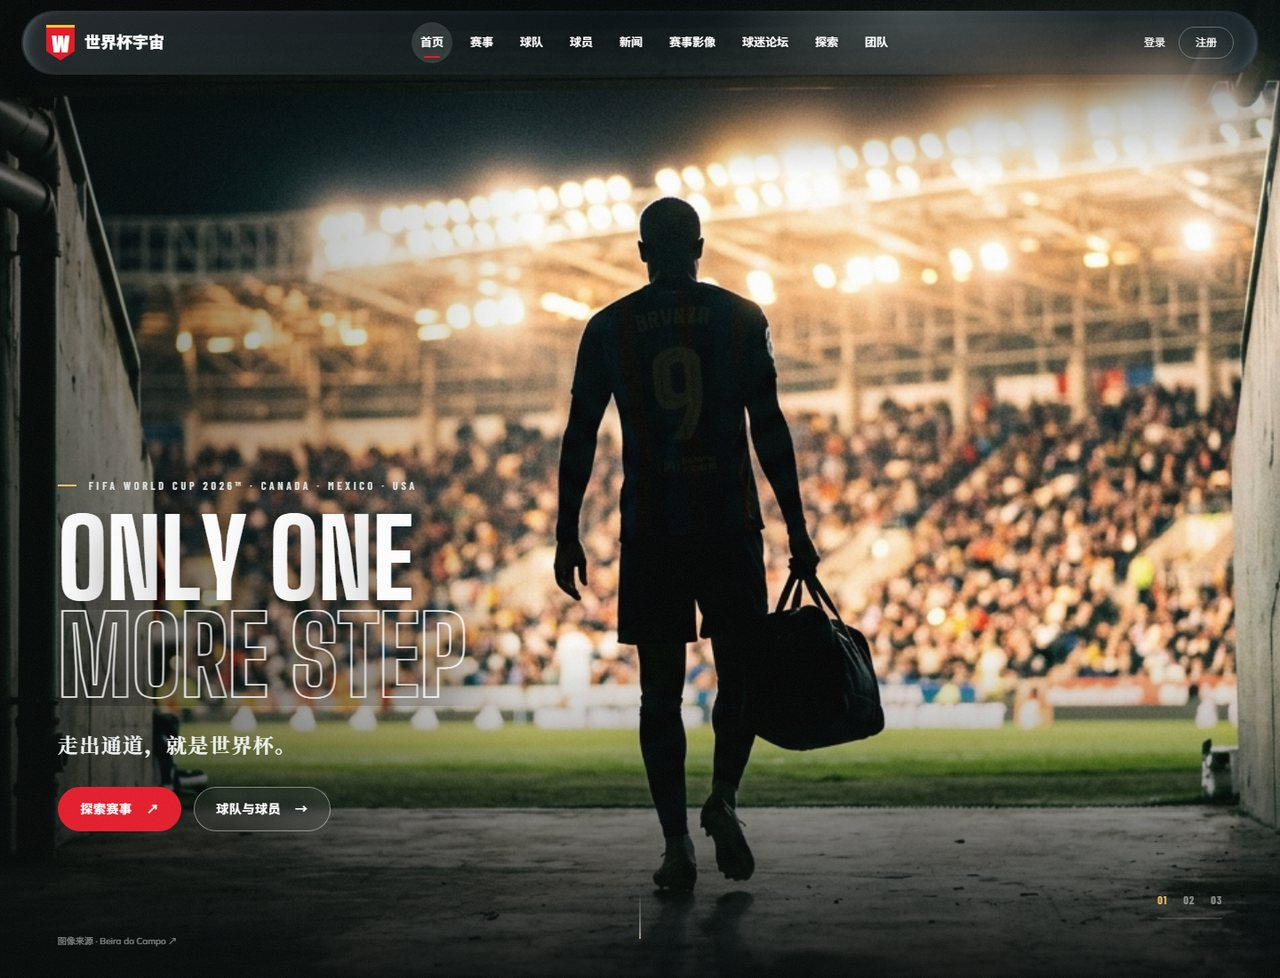
\includegraphics[width=\textwidth]{screenshots/home.jpg}
\caption{网站首页}
\end{figure}

\Needspace{7\baselineskip}
\subsection{表单反馈}
发布主题、填写注册表单、编辑用户资料和管理后台记录均由对应模型校验属性。控制器把字段错误交给视图呈现，用户可在原页面修改内容。成功的创建或保存通常使用重定向，减少表单重复提交。

业务状态采用明确的字符串标识：论坛主题以 published、hidden、deleted 等状态区分可见性，新闻以 draft、published、hidden 区分发布情况，留言默认 pending，需要管理员审核后公开。

\section{命令行安装入口}
管理员可运行 php yii app/install 建立基础数据库与迁移记录。命令初始化管理员和系统角色，检测已有体育数据后避免重复写入基础种子。新环境必须在 .env 指定数据库参数及管理员初始密码。

已有数据的服务器升级应保留 .env、上传文件和数据库数据，运行部署脚本时按迁移记录更新结构。管理员密码重置通过单独的控制台命令执行，通过控制台命令更新账户密码哈希及认证密钥。

\Needspace{7\baselineskip}
\subsection{本地和服务器部署}
Windows 端的 deploy-local.bat 用于配置本地完整工程，启动 PHP 内置 Web 服务及数据库。Linux 端 scripts/deploy.sh 安装 Nginx、PHP-FPM、MariaDB 和证书工具，再生成相应系统配置。两种运行方式使用相同 Yii2 代码与数据结构。

生产脚本通过 flock 文件锁限制并发部署，先执行环境与依赖检查，再更新配置与迁移。服务器的运行数据目录和代码目录分离，自动更新保留运行记录。

\Needspace{7\baselineskip}
\subsection{定时任务}
仓库的部署说明记载：生产服务器定时检查 main 分支的新提交，升级前备份数据库和文件，部署成功后执行健康检查。新闻同步、备份与证书续期分别由系统定时服务负责。

备份文件包含运行时数据库与实际上传内容，与代码版本分别保存。Git 负责代码版本，数据库备份负责用户内容和变化中的记录。两种恢复路径分别对应程序版本和运行数据。


\Needspace{16\baselineskip}
\noindent\textbf{commands/NewsController.php：新闻同步命令}\par\vspace{2pt}
\begin{lstlisting}
public function actionSync(): int
{
    $result=(new \app\services\NewsImportService())->sync();
    $this->stdout(gmdate(DATE_ATOM).' '.json_encode(
        $result,JSON_PRETTY_PRINT|JSON_UNESCAPED_UNICODE)."\n");
    if (!empty($result['busy'])) { return 0; }
    $failed=array_column(array_filter($result['sources'],
        static fn(array $s):bool=>$s['status']==='failed'),'name');
    if ($failed) {
        \Yii::error('News sources failed: '.implode(', ',$failed),'news');
    }
    return count($result['sources'])-count($failed)>0?0:1;
}
\end{lstlisting}

\section{Git 提交记录}
项目使用 Git 维护代码版本，通过 GitHub main 分支汇集开发提交。提交 cf285427 更新了新闻同步命令、新闻导入服务和页面视图；3d37b678 修改新闻刷新逻辑及前端脚本。其他提交涉及论坛页面整理、视频目录和交付文件。主要提交与修改文件列于下表。

\begin{longtable}{>{\raggedright\arraybackslash}p{.28\textwidth}>{\raggedright\arraybackslash}p{.64\textwidth}}\toprule 项目 & 说明\\\midrule\endfirsthead\toprule 项目 & 说明\\\midrule\endhead
cf285427 & 修改 commands/NewsController.php、services/NewsImportService.php 和新闻视图\\\midrule
3d37b678 & 修改新闻控制器、新闻同步服务与 news-live.js\\\midrule
1346165b & 更新 docs/implementation.md 及 data/team 内实现文档 PDF、DOCX\\\midrule
8f8f0217 & 更新实现文档交付文件与 Markdown 原稿\\\midrule
37f167cd & 更新实现文档交付文件与 Markdown 原稿\\\midrule
4348c69a & 更新 README 和论坛整理证据文件\\\midrule
7766f3e9 & 更新 README 和网站健康检查材料\\\midrule
0730a13d & 调整视频控制器、视频配置和视频目录迁移\\\midrule
\bottomrule\caption{可追溯提交记录}\end{longtable}
\Needspace{7\baselineskip}
\subsection{团队分工}
团队由崔迪（2412439）、梁靖泽（2412852）、蒋林瀞（2413507）、王麒萱（2412096）组成。项目原型中的任务安排为前台信息架构、赛事内容、后台管理、界面原型及报告。具体页面按照赛事、社区、后台和部署模块组织，成员通过 GitHub 协作更新代码及资料。

项目代码主要通过 Aqs-1733 仓库维护。各业务模块的模型、视图和控制器按功能目录保存，具体文件分布列于下表。

\Needspace{7\baselineskip}
\subsection{MVC 文件分布}
球队、赛事、论坛、个人中心及后台采用相同的 MVC 组织方式。控制器负责路由和请求，模型管理数据字段及关联，服务层编写业务事务，视图负责页面布局。

\begin{longtable}{>{\raggedright\arraybackslash}p{.28\textwidth}>{\raggedright\arraybackslash}p{.64\textwidth}}\toprule 项目 & 说明\\\midrule\endfirsthead\toprule 项目 & 说明\\\midrule\endhead
赛事 & controllers/MatchController.php；models/MatchGame.php；views/catalog/ 下赛事视图；services/CatalogService.php\\\midrule
球队 & controllers/TeamController.php；models/Team.php；views/catalog/teams.php 和 team.php\\\midrule
球员 & controllers/PlayerController.php；models/Player.php；views/catalog/ 下球员页面\\\midrule
论坛 & controllers/ForumController.php；models/ForumThread.php、ForumReply.php；views/forum/；services/ForumService.php\\\midrule
个人中心 & controllers/ProfileController.php；models/FanProfile.php；views/profile/；services/PreferenceService.php\\\midrule
后台管理 & controllers/AdminController.php；models/AuditLog.php 等；views/admin-v2/\\\midrule
新闻 & controllers/NewsController.php；models/NewsArticle.php；views/catalog/news.php；services/NewsImportService.php\\\midrule
\bottomrule\caption{主要 MVC 文件对应表}\end{longtable}
\section{页面功能对应}
前台以赛事、球队、国家、新闻、论坛及个人中心组成主要访问路径，后台负责数据编辑和社区管理。页面控制器分别读取业务记录并把查询结果传入对应视图。

赛事页面可按阶段筛选比赛，球队页面支持名称搜索，论坛页面可以创建主题并回复，管理员界面提供数据编辑入口。

\section{实现总结}
世界杯宇宙围绕赛事资料建立了统一的数据库。球队、球员、比赛、阵容和积分通过主外键关联，浏览者可从赛程进入比赛详情，再进入球队或球员资料。国家探索、新闻和回放页面补充赛事相关内容，前台按照不同场景提供搜索、筛选和分页。

账号注册使用模型校验、密码哈希及会话认证。用户设置主队、关注球队和球员时，使用事务更新个人资料及关联表。论坛主题和回复按作者身份保存，回复通知随业务写入一同提交。管理员通过白名单控制数据维护范围，并记录关键操作的审计信息。

体育数据使用官方来源采集快照和 SHA256 保存来源记录；新闻采集按来源同步并维护文章发布状态。工程还配有数据库安装、增量迁移、Windows 本地启动和公网部署，便于按照同一份源码运行各业务模块。

\section{主要文件索引}
\begin{longtable}{p{.31\textwidth}p{.60\textwidth}}\toprule 路径 & 内容\\\midrule\endfirsthead\toprule 路径 & 内容\\\midrule\endhead
config/web.php & 路由、会话、CSRF 及应用组件配置\\\midrule
controllers/ & 赛事、账号、论坛、个人中心和管理后台控制器\\\midrule
models/ & 数据库实体、模型规则与关联查询\\\midrule
services/ & 业务事务、体育数据导入、新闻同步、媒体上传和操作审计\\\midrule
views/ & 前台页面、后台页面及公共布局\\\midrule
commands/ & 数据安装、体育数据导入、新闻同步命令\\\midrule
migrations/ & Yii2 数据库增量迁移\\\midrule
data/install.sql & 数据库基础建表语句\\\midrule
data/official/20261021/ & 体育数据来源文件、采集清单和规范化数据\\\midrule
\bottomrule\caption{工程主要文件}\end{longtable}

\section{参考资料}
\begin{enumerate}[label={[\arabic*]},leftmargin=3em]
\item FIFA. FIFA World Cup 2026. \url{https://www.fifa.com/fifaplus/en/tournaments/mens/worldcup/canadamexicousa2026}
\item Yii Software LLC. Yii 2.0 Definitive Guide. \url{https://www.yiiframework.com/doc/guide/2.0/en}
\item PHP Documentation Group. PHP Manual. \url{https://www.php.net/manual/zh/}
\item MariaDB Foundation. MariaDB Server Documentation. \url{https://mariadb.com/kb/en/documentation/}
\item BBC Sport. Football RSS. \url{https://feeds.bbci.co.uk/sport/football/rss.xml}
\item ESPN. Soccer RSS. \url{https://www.espn.com/espn/rss/soccer/news}
\item 中国新闻网. 体育频道. \url{https://www.chinanews.com.cn/sports/}
\end{enumerate}
项目地址：\url{https://github.com/Aqs-1733/worldcup-universe}。


\end{document}